\documentclass[11pt, a4paper]{article}

\usepackage[a4paper, margin=2.5cm]{geometry}
\usepackage[utf8]{inputenc}
\usepackage[T1]{fontenc}
\usepackage[english]{babel}
\usepackage{lmodern}
\usepackage{enumitem}
\setlist[itemize]{label=-}
\usepackage{booktabs}
\usepackage{graphicx} % Hozzáadva a nagyméretű UML ábrák szélességének auto-skálázásához
\usepackage{tikz} % Added for the FSM diagram
\usetikzlibrary{shapes.multipart, positioning, arrows.meta} % Added for UML Diagram
\usepackage[colorlinks=true, linkcolor=black, urlcolor=blue]{hyperref}
% Long \texttt names cannot be hyphenated; allow a little extra word spacing instead of running into the margin
\setlength{\emergencystretch}{3em}

\usepackage{fancyhdr}
\pagestyle{fancy}
\fancyhf{}
\lhead{\textbf{PAC-MAN}}
\rhead{Balázs Tari}
\cfoot{\thepage}
\renewcommand{\headrulewidth}{0.4pt}

\begin{document}

% --- Title Page ---
\begin{titlepage}
    \centering
    \vspace*{4cm}
    {\Huge \textbf{PAC-MAN} \par}
    \vspace{1.5cm}
    {\LARGE Basics of Programming 3. \par}
    \vspace{0.5cm}
    {\Large Project Specification \par}
    
    \vspace{4.5cm}
    
    {\Large \textbf{Balázs Tari} \par}
    \vspace{0.3cm}
    {\Large E3K6W5 \par}
    
    \vfill
    
    {\large October 16, 2026 \par}
    \vspace{0.2cm}
    {\normalsize Revised: November 6, 2026 \par}
\end{titlepage}

% --- Table of Contents ---
\tableofcontents
\newpage

% --- 1. Task Description ---
\section{Task Description}
Pac-Man is a two-dimensional desktop arcade game. The player controls the yellow figure in a labyrinth, whose task is to collect all dots while avoiding the ghosts moving around the map. If Pac-Man collects one of the 4 'Power Pellets' located in the labyrinth, the player gains the ability to eat ghosts for 6 seconds, earning additional points. 

The software's graphical user interface is built using the Java Swing framework, the persistent storage of the game state is managed via file handling, and the code quality is ensured by automated JUnit unit tests.

% --- 2. Use-Cases ---
\section{Use-Cases}
\begin{enumerate}
    \item \textbf{Starting and controlling the game:} The user can start a new game from the menu and control Pac-Man within the labyrinth using the WASD keyboard keys.
    \item \textbf{Collecting dots and victory:} As Pac-Man passes through the dots, they disappear, and the score increases. If all dots are consumed, the player wins and proceeds to the next level. At higher levels, the difficulty of the game increases.
    \item \textbf{Collision detection with ghosts:} If the character collides with a ghost, it loses a life. If the number of lives reaches zero, the game ends (Game Over). Upon starting a new game, the player always begins at the first level.
    \item \textbf{Saving high-scores:} At the end of a game, the system records and saves the achieved score to a file.
    \item \textbf{Saving game state:} The game can be saved at any time and state, allowing the player to load and resume it later from a file.
    \item \textbf{Level editor mode:} In addition to the base game, the user has the ability to design their own custom maps, save them, and load previously created maps to play on.
\end{enumerate}

% --- 3. Solution Overview ---
\section{Solution Overview}
\begin{enumerate}
    \item \textbf{Applied technological solutions:} Java SE, Swing (JFrame, JPanel, Graphics for low-level drawing, \texttt{javax.swing.Timer} driving the game loop at 60 ticks per second), and JUnit 5 for automated testing.
    \item \textbf{File formats:} A simple CSV file for storing the high-score table, a plain-text tile picture (one character per tile) for map layouts, and Java binary serialization for saved game states.
\end{enumerate}

\clearpage

% --- 4. Detailed Architecture and Class Structure ---
\section{Detailed Architecture and Class Structure}

\textbf{Core Game Model}
\begin{itemize}
    \item \textbf{GameEngine:} The central controller of the game. It runs the game loop (see Section~\ref{sec:game_loop}), updates the game state (positions, collisions), and manages the score, remaining lives, and the \texttt{currentLevel}. It is also responsible for saving and loading the active game state (utilizing \texttt{java.io.Serializable}). As the level increases, the duration of the ghosts' Frightened state progressively decreases to increase difficulty; the normal movement speed of Pac-Man and the ghosts stays the same on every level. A new game is started from a \texttt{LevelData} object built by the \texttt{LevelManager}, always with score 0, 3 lives, and level 1. The engine owns one shared \texttt{java.util.Random} for the ghosts' random choices; a second constructor accepts a given \texttt{Random}, so tests can pass a fixed seed and get the same choices on every run.
    \item \textbf{Labyrinth:} The class representing the map. It stores the type of every tile (wall, dot, power pellet, empty) in a two-dimensional array, indexed as \texttt{grid[row][column]}. A tile is walkable if it is not a wall, and any position outside the array counts as a wall, so nothing can leave the map. An intersection is a walkable tile with at least three walkable neighbours. The \texttt{Labyrinth} does not read files; levels are loaded by the \texttt{LevelManager}.
    \item \textbf{GameObject} (Abstract Base Class): Encapsulates common properties for all moving entities (X and Y coordinates, speed, direction). Positions are \textbf{tile coordinates}: \texttt{x} is the column and \texttt{y} is the row of the maze, and \texttt{speed} is the number of whole tiles one step covers. Besides the current tile, every object remembers two more:
    \begin{itemize}
        \item its \textbf{start tile} (\texttt{startX}, \texttt{startY}, \texttt{final}), where \texttt{resetToStart()} puts it back after Pac-Man loses a life, standing still;
        \item its \textbf{previous tile} (\texttt{prevX}, \texttt{prevY}), saved by \texttt{rememberPosition()} at the start of every step, even if the object does not move. The view uses it to slide the figure smoothly between two tiles, and the collision check uses it to detect two figures passing through each other.
    \end{itemize}
    \begin{itemize}
        \item \textbf{PacMan} (Child Class): Represents the state of the player's character and handles its input logic: the latest key press is buffered as a \texttt{Command} and run at the next step. It overrides \texttt{resetToStart()}: after calling the parent version it also drops the buffered command, so a key pressed before dying does not start Pac-Man moving again right away.
        \item \textbf{Ghost} (Child Class): Represents the state of the ghosts and manages their movement. \texttt{possibleDirections()} lists the walkable directions from the current tile, without turning back, unless the ghost is in a dead end. Two methods pick one of them: \texttt{chooseDirection()} picks at random, \texttt{chooseDirectionTowards(target)} picks the direction whose next tile is closest to a target tile (see Section~\ref{sec:game_loop}). \texttt{chooseChaseDirection()} asks the ghost's strategy object for the target (see Section~\ref{sec:design_patterns}) and steps towards it; a ghost whose personality has no strategy yet falls back to the random pick. In a corridor or a corner only one direction is left, so a real choice only happens at intersections. State changes are triggered by events, each with its own method: \texttt{frighten()}, \texttt{calmDown()}, \texttt{eaten()} and \texttt{respawn()}. The ghost also overrides \texttt{resetToStart()}: after the parent version it sets the state back to \texttt{CHASE}, so after Pac-Man loses a life no ghost stays frightened or dead.
    \end{itemize}
    \item \textbf{LevelData:} A plain data holder for the content of one map file: the \texttt{Labyrinth}, Pac-Man on his start tile, and the ghosts on their start tiles. The \texttt{LevelManager} creates it, and the \texttt{GameEngine} is built from its parts.
\end{itemize}

\vspace{0.3cm}
\textbf{UI and Management Classes}
\begin{itemize}
    \item \textbf{MainFrame (JFrame):} The application's main window utilizing a CardLayout to switch between the menu, the active game, and the editor.
    \item \textbf{MainMenu (JPanel):} The start screen providing options to start a new game, load a saved game, view high scores, or open the map editor.
    \item \textbf{GamePanel (JPanel):} The active gameplay screen that bridges the Model and View. It turns WASD key presses into \texttt{MoveCommand} objects, receives the game state from the \texttt{GameEngine}, and renders the maze and entities in its \texttt{paintComponent} method. Figures are drawn between their previous and current tile according to the engine's step progress, so movement looks smooth although the model works in whole tiles. A ghost's colour shows its personality (\texttt{TRACKER} red, \texttt{AMBUSHER} pink, \texttt{WANDERER} orange, \texttt{CHAOTIC} cyan, so it stays visible next to the dark blue walls). The state wins over the personality: a frightened ghost is white, and a \texttt{DEAD} ghost is only a small grey dot (its eyes). The heads-up line shows the score, the remaining lives, and \texttt{GAME OVER} when no life is left.
    \item \textbf{MapEditor (JPanel):} A graphical interface with a clickable grid allowing the user to draw custom mazes (placing walls, dots, power pellets, Pac-Man's start tile, and the start tiles of the four ghosts).
    \item \textbf{LevelManager (Factory):} A dedicated, stateless class that reads a map file into a \texttt{LevelData} (maze, Pac-Man, and ghosts) and writes a \texttt{LevelData} back to a map file in the same format (see Section~\ref{sec:custom_maps}). It also manages the high-score table.
\end{itemize}


\begin{figure}[h!]
    \centering
    \resizebox{\textwidth}{!}{ % Ráhúzza a diagramot a maximális lapszélességre
    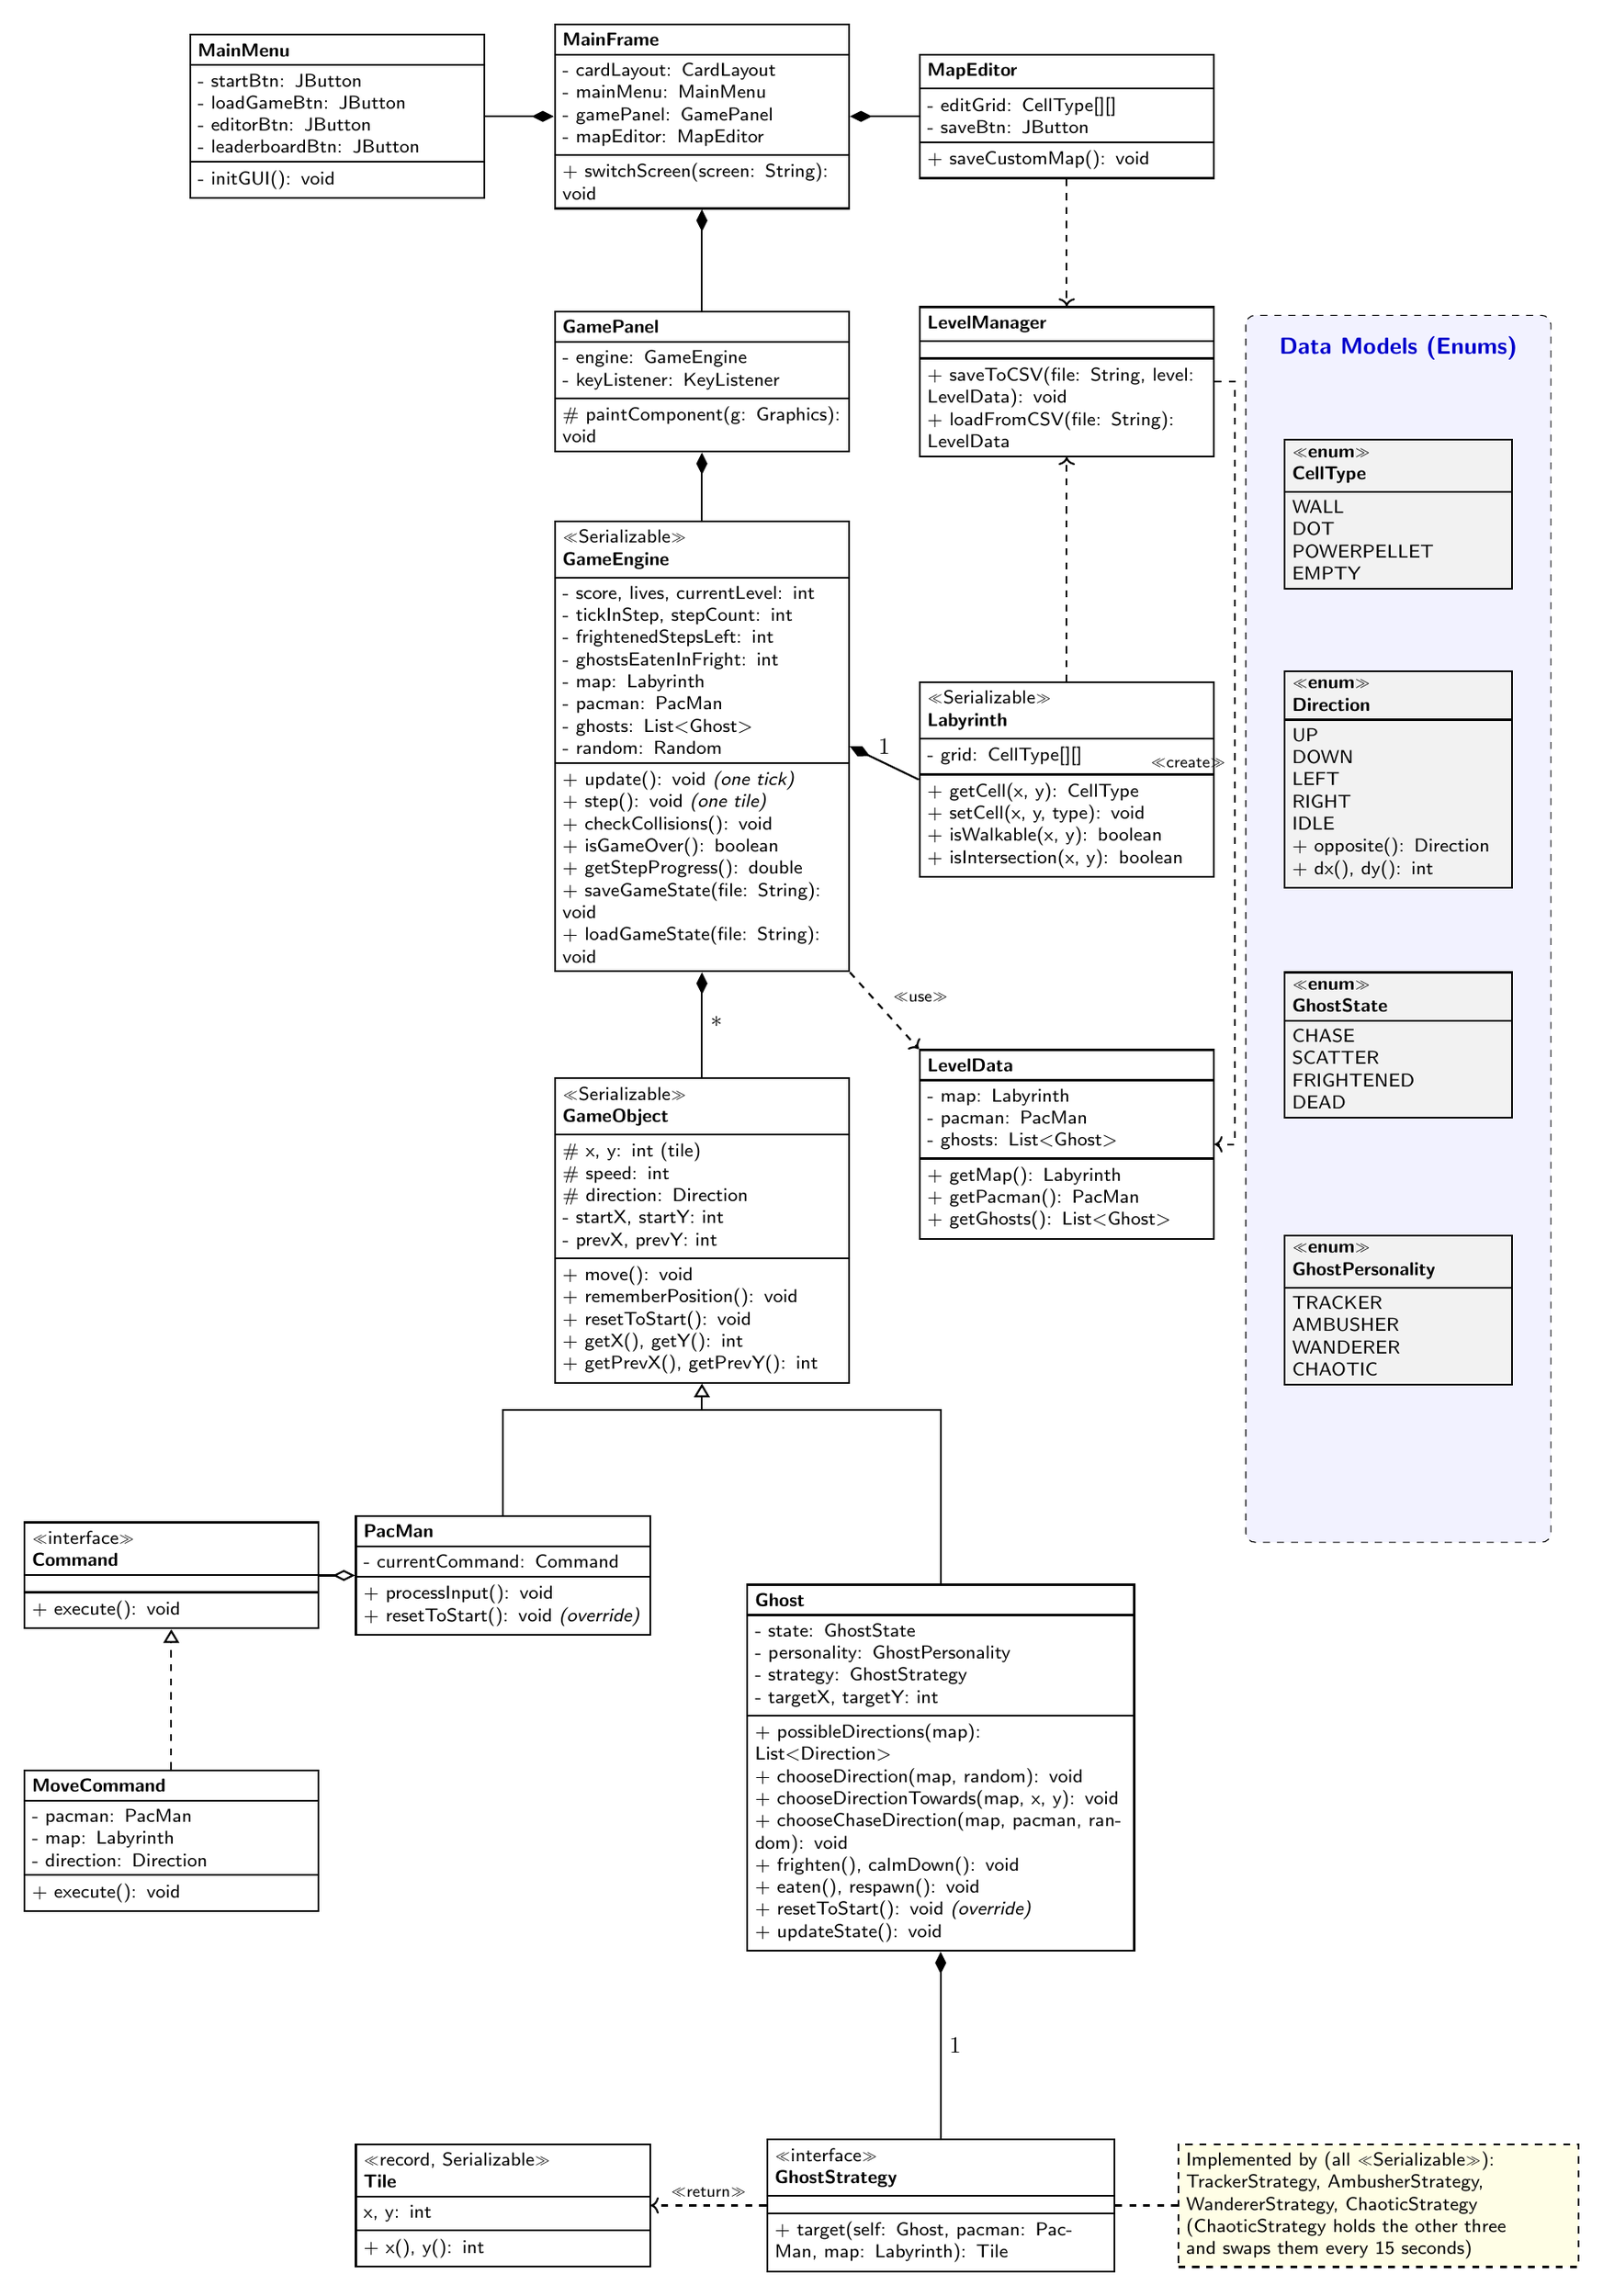
\begin{tikzpicture}[
        umlclass/.style={
            draw, thick,
            rectangle split,
            rectangle split parts=3,
            font=\sffamily\footnotesize, % Olvashatóbb, nagyobb betűméret
            align=left,
            text width=4.2cm,
            fill=white
        },
        umlenum/.style={
            draw, thick,
            rectangle split,
            rectangle split parts=2,
            font=\sffamily\footnotesize,
            align=left,
            text width=3.2cm,
            fill=gray!10
        }
    ]
        
        % === UI & MANAGEMENT LAYER ===
        \node[umlclass] (MainFrame) at (0, 7.5) {
            \textbf{MainFrame}
            \nodepart{two}
            - cardLayout: CardLayout \\
            - mainMenu: MainMenu \\
            - gamePanel: GamePanel \\
            - mapEditor: MapEditor
            \nodepart{three}
            + switchScreen(screen: String): void
        };

        \node[umlclass] (MainMenu) at (-5.5, 7.5) {
            \textbf{MainMenu}
            \nodepart{two}
            - startBtn: JButton \\
            - loadGameBtn: JButton \\
            - editorBtn: JButton \\
            - leaderboardBtn: JButton
            \nodepart{three}
            - initGUI(): void
        };

        \node[umlclass] (MapEditor) at (5.5, 7.5) {
            \textbf{MapEditor}
            \nodepart{two}
            - editGrid: CellType[][] \\
            - saveBtn: JButton
            \nodepart{three}
            + saveCustomMap(): void
        };

        \node[umlclass] (LevelManager) at (5.5, 3.5) {
            \textbf{LevelManager}
            \nodepart{two}
            % Nincs belső állapot (Utility/Factory)
            \nodepart{three}
            + saveToCSV(file: String, level: LevelData): void \\
            + loadFromCSV(file: String): LevelData
        };

        \node[umlclass] (GamePanel) at (0, 3.5) {
            \textbf{GamePanel}
            \nodepart{two}
            - engine: GameEngine \\
            - keyListener: KeyListener
            \nodepart{three}
            \# paintComponent(g: Graphics): void
        };


        % === CORE MODEL LAYER ===
        \node[umlclass] (GameEngine) at (0, -2.0) {
            \guillemotleft Serializable\guillemotright \\
            \textbf{GameEngine}
            \nodepart{two}
            - score, lives, currentLevel: int \\
            - tickInStep, stepCount: int \\
            - frightenedStepsLeft: int \\
            - ghostsEatenInFright: int \\
            - map: Labyrinth \\
            - pacman: PacMan \\
            - ghosts: List$<$Ghost$>$ \\
            - random: Random
            \nodepart{three}
            + update(): void \textit{(one tick)} \\
            + step(): void \textit{(one tile)} \\
            + checkCollisions(): void \\
            + isGameOver(): boolean \\
            + getStepProgress(): double \\
            + saveGameState(file: String): void \\
            + loadGameState(file: String): void
        };

        \node[umlclass] (Labyrinth) at (5.5, -2.5) {
            \guillemotleft Serializable\guillemotright \\
            \textbf{Labyrinth}
            \nodepart{two}
            - grid: CellType[][]
            \nodepart{three}
            + getCell(x, y): CellType \\
            + setCell(x, y, type): void \\
            + isWalkable(x, y): boolean \\
            + isIntersection(x, y): boolean
        };

        \node[umlclass] (GameObject) at (0, -9.3) {
            \guillemotleft Serializable\guillemotright \\
            \textbf{\textit{GameObject}}
            \nodepart{two}
            \# x, y: int (tile) \\
            \# speed: int \\
            \# direction: Direction \\
            - startX, startY: int \\
            - prevX, prevY: int
            \nodepart{three}
            + move(): void \\
            + rememberPosition(): void \\
            + resetToStart(): void \\
            + getX(), getY(): int \\
            + getPrevX(), getPrevY(): int
        };

        \node[umlclass] (PacMan) at (-3, -14.5) {
            \textbf{PacMan}
            \nodepart{two}
            - currentCommand: Command
            \nodepart{three}
            + processInput(): void \\
            + resetToStart(): void \textit{(override)}
        };
        
        \node[umlclass] (Command) at (-8, -14.5) {
            \guillemotleft interface\guillemotright \\
            \textbf{Command}
            \nodepart{two}
            \nodepart{three}
            + execute(): void
        };

        \node[umlclass, text width=5.6cm] (Ghost) at (3.6, -17.4) {
            \textbf{Ghost}
            \nodepart{two}
            - state: GhostState \\
            - personality: GhostPersonality \\
            - strategy: GhostStrategy \\
            - targetX, targetY: int
            \nodepart{three}
            + possibleDirections(map): List$<$Direction$>$ \\
            + chooseDirection(map, random): void \\
            + chooseDirectionTowards(map, x, y): void \\
            + chooseChaseDirection(map, pacman, random): void \\
            + frighten(), calmDown(): void \\
            + eaten(), respawn(): void \\
            + resetToStart(): void \textit{(override)} \\
            + updateState(): void
        };

        \node[umlclass] (MoveCommand) at (-8, -18.5) {
            \textbf{MoveCommand}
            \nodepart{two}
            - pacman: PacMan \\
            - map: Labyrinth \\
            - direction: Direction
            \nodepart{three}
            + execute(): void
        };

        \node[umlclass] (LevelData) at (5.5, -8.0) {
            \textbf{LevelData}
            \nodepart{two}
            - map: Labyrinth \\
            - pacman: PacMan \\
            - ghosts: List$<$Ghost$>$
            \nodepart{three}
            + getMap(): Labyrinth \\
            + getPacman(): PacMan \\
            + getGhosts(): List$<$Ghost$>$
        };

        \node[umlclass, text width=5.0cm] (GhostStrategy) at (3.6, -24.0) {
            \guillemotleft interface\guillemotright \\
            \textbf{GhostStrategy}
            \nodepart{two}
            \nodepart{three}
            + target(self: Ghost, pacman: PacMan, map: Labyrinth): Tile
        };

        \node[umlclass] (Tile) at (-3, -24.0) {
            \guillemotleft record, Serializable\guillemotright \\
            \textbf{Tile}
            \nodepart{two}
            x, y: int
            \nodepart{three}
            + x(), y(): int
        };

        \node[draw, dashed, thick, font=\sffamily\footnotesize, align=left, text width=5.8cm, fill=yellow!10] (StrategyNote) at (10.2, -24.0) {
            Implemented by (all \guillemotleft Serializable\guillemotright): \\
            TrackerStrategy, AmbusherStrategy, \\
            WandererStrategy, ChaoticStrategy \\
            (ChaoticStrategy holds the other three \\
            and swaps them every 15 seconds)
        };

        % === DATA MODELS (ENUMS) SZUPERÁLT BLOKK ===
        % Dedikált, halvány hátterű keret az Enumoknak
       \draw[dashed, fill=blue!5, rounded corners] (8.2, 4.5) rectangle (12.8, -14.0);
        \node[font=\sffamily\bfseries, text=blue!80!black] at (10.5, 4.0) {Data Models (Enums)};

        \node[umlenum] (CellType) at (10.5, 1.5) {
            \textbf{\guillemotleft enum\guillemotright \\ CellType}
            \nodepart{two}
            WALL \\ DOT \\ POWERPELLET \\ EMPTY
        };

        \node[umlenum] (Direction) at (10.5, -2.5) {
            \textbf{\guillemotleft enum\guillemotright \\ Direction}
            \nodepart{two}
            UP \\ DOWN \\ LEFT \\ RIGHT \\ IDLE \\
            + opposite(): Direction \\
            + dx(), dy(): int
        };

        \node[umlenum] (GhostState) at (10.5, -6.5) {
            \textbf{\guillemotleft enum\guillemotright \\ GhostState}
            \nodepart{two}
            CHASE \\ SCATTER \\ FRIGHTENED \\ DEAD
        };

        \node[umlenum] (GhostPersonality) at (10.5, -10.5) {
            \textbf{\guillemotleft enum\guillemotright \\ GhostPersonality}
            \nodepart{two}
            TRACKER \\ AMBUSHER \\ WANDERER \\ CHAOTIC
        };

        % === RELATIONSHIPS ===
        % UI dependenciák és kompozíciók
        \draw[{Diamond[fill=black, scale=1.2]}-, thick] (MainFrame.west) -- (MainMenu.east);
        \draw[{Diamond[fill=black, scale=1.2]}-, thick] (MainFrame.east) -- (MapEditor.west);
        \draw[{Diamond[fill=black, scale=1.2]}-, thick] (MainFrame.south) -- (GamePanel.north);
        
        \draw[dashed, ->, thick] (MapEditor.south) -- (LevelManager.north);
        \draw[dashed, ->, thick] (Labyrinth.north) -- (LevelManager.south);
        \draw[{Diamond[fill=black, scale=1.2]}-, thick] (GamePanel.south) -- (GameEngine.north);

        % Model kapcsolatok
        \draw[{Diamond[fill=black, scale=1.2]}-, thick] (GameEngine.east) -- (Labyrinth.west) node[midway, above] {1};
        \draw[{Diamond[fill=black, scale=1.2]}-, thick] (GameEngine.south) -- (GameObject.north) node[midway, right] {*};

        % Öröklődés (Inheritance)
        \draw[-{Triangle[open, fill=white, scale=1.2]}, thick] ([yshift=-0.4cm]GameObject.south) -- (GameObject.south);
        \draw[thick] (PacMan.north) |- ([yshift=-0.4cm]GameObject.south);
        \draw[thick] (Ghost.north) |- ([yshift=-0.4cm]GameObject.south);
        
        % Command pattern aggregáció
        \draw[{Diamond[fill=white, scale=1.2]}-, thick] (PacMan.west) -- (Command.east);
        % MoveCommand realizes Command
        \draw[dashed, -{Triangle[open, fill=white, scale=1.2]}, thick] (MoveCommand.north) -- (Command.south);

        % LevelData: LevelManager creates it, GameEngine is built from it
        \draw[dashed, ->, thick] (LevelManager.east) -- ++(0.3, 0) |- (LevelData.east) node[pos=0.25, left, font=\sffamily\scriptsize] {\guillemotleft create\guillemotright};
        \draw[dashed, ->, thick] (GameEngine.south east) -- (LevelData.north west) node[midway, above right, font=\sffamily\scriptsize] {\guillemotleft use\guillemotright};

        % Strategy pattern: the ghost owns its strategy object
        \draw[{Diamond[fill=black, scale=1.2]}-, thick] (Ghost.south) -- (GhostStrategy.north) node[midway, right] {1};
        \draw[dashed, thick] (GhostStrategy.east) -- (StrategyNote.west);
        \draw[dashed, ->, thick] (GhostStrategy.west) -- (Tile.east) node[midway, above, font=\sffamily\scriptsize] {\guillemotleft return\guillemotright};

    \end{tikzpicture}
    } % \resizebox vége
    \caption{UML Class Diagram of the Complete Game Architecture}
    \label{fig:uml_complete_diagram}
\end{figure}

\clearpage

\subsection{Game Loop, Movement and Collisions}
\label{sec:game_loop}
The model works in whole tiles, but the screen is redrawn 60 times per second. The two are kept apart by separating a \textit{tick} from a \textit{step}:
\begin{itemize}
    \item \textbf{Tick:} The Swing \texttt{Timer} in the \texttt{GamePanel} fires every $1000 / \texttt{TICKS\_PER\_SECOND}$ ms ($\approx$16 ms), calls \texttt{GameEngine.update()}, then \texttt{repaint()}. One \texttt{update()} is one tick.
    \item \textbf{Step:} Every \texttt{TICKS\_PER\_STEP} (= 10) ticks, \texttt{update()} calls \texttt{step()}, which moves every figure by at most one tile. With 60 ticks per second this is 6 tiles per second. All game rules (input, movement, collisions, scoring) run in \texttt{step()}, so the unit tests call \texttt{step()} directly and do not depend on timing.
    \item \textbf{Smooth drawing (interpolation):} \texttt{getStepProgress()} returns how far the current step is, between 0.0 and 1.0. The \texttt{GamePanel} draws each figure at $(\textit{previous} + (\textit{current} - \textit{previous}) \cdot \textit{progress}) \cdot \textit{TILE}$ pixels. The pixel calculation lives only in the view; the model never deals with pixels. As a side effect the picture runs up to one step ($\approx$166 ms) behind the model.
    \item \textbf{Durations:} Every duration (Frightened time, the Chaotic ghost's 15-second switch) is converted from seconds with \texttt{TICKS\_PER\_SECOND}, so changing the tick rate needs only one constant.
\end{itemize}

\textbf{Order of one step:}
\begin{enumerate}
    \item If the game is over, nothing happens.
    \item Pac-Man runs his buffered command, which turns him if the tile in the wished direction is open, then steps one tile unless a wall is ahead.
    \item If the frightened timer is running, it counts down by one; when it reaches 0, every ghost gets \texttt{calmDown()}. This happens before anyone moves, so in that step the ghosts already move at full speed.
    \item Pac-Man runs his buffered command, which turns him if the tile in the wished direction is open, then steps one tile unless a wall is ahead.
    \item Each ghost chooses a direction according to its state and steps:
    \begin{itemize}
        \item \texttt{DEAD}: towards its own start tile in the Ghost House (\texttt{chooseDirectionTowards});
        \item \texttt{FRIGHTENED}: at random, and only on every \texttt{FRIGHTENED\_STEP\_INTERVAL} (= 2) steps, so it is half as fast; on the skipped steps it still calls \texttt{rememberPosition()};
        \item otherwise: towards the target of its strategy (\texttt{chooseChaseDirection}).
    \end{itemize}
    After its step, \texttt{respawn()} turns a \texttt{DEAD} ghost that has just reached its start tile back into \texttt{CHASE}. Calling it after the step matters: a ghost eaten on its own start tile first has to leave it, otherwise it would come back to life at once.
    \item Collisions are checked once everyone has moved.
\end{enumerate}
Before moving, every figure saves its previous tile with \texttt{rememberPosition()}, even if it stands still. Otherwise the view would replay the last slide and the collision check would compare old tiles.

\textbf{Ghost movement rules:} A ghost never turns back by 180 degrees, except in a dead end, where turning back is the only way out, and once when it becomes frightened. In a corridor or a corner only one direction is left, so a ghost really decides only at intersections.

\textbf{Target Tile Routing:} \texttt{chooseDirectionTowards(target)} looks at every direction from \texttt{possibleDirections()} and picks the one whose next tile is closest to the target. It is a \textit{greedy} choice: the best-looking step now, without planning ahead, exactly as in the original game. It does not always find the shortest path, which makes the ghosts predictable but not perfect. The distance is the squared straight-line distance $dx^2 + dy^2$; the square root is skipped, because it does not change which distance is smaller, so the calculation stays in integers. On a tie, the direction that comes first in the list (\texttt{UP}, \texttt{DOWN}, \texttt{LEFT}, \texttt{RIGHT}) wins. The target may lie on a wall or outside the maze; it only has to be measurable, not reachable. The chosen target is stored in \texttt{targetX}, \texttt{targetY}.

\textbf{Collisions:}
\begin{itemize}
    \item \textbf{Dots and power pellets:} If Pac-Man ends a step on a \texttt{DOT} (10 points) or a \texttt{POWERPELLET} (50 points), the score increases and the tile becomes \texttt{EMPTY}. A power pellet also calls \texttt{frighten()} on every ghost, (re)starts the frightened timer, and resets the ghost-eating series.
    \item \textbf{Frightened duration:} \texttt{frightenedDurationSteps()} reads the duration from the current level and converts it to steps ($\textit{seconds} \cdot \texttt{TICKS\_PER\_SECOND} / \texttt{TICKS\_PER\_STEP}$, multiplying first so integer division cannot cut off a fraction):

    \vspace{0.1cm}
    \begin{tabular}{@{}lll@{}}
        \toprule
        \textbf{Level} & \textbf{Seconds} & \textbf{Steps} \\
        \midrule
        1--3 & 6 & 36 \\
        4--6 & 4 & 24 \\
        7--10 & 2 & 12 \\
        11+ & 1 & 6 \\
        \bottomrule
    \end{tabular}
    \vspace{0.1cm}

    The duration never reaches 0: a 0-step fright would turn the ghosts white and around, and the countdown could leave them frightened forever. A new pellet restarts the full duration.
    \item \textbf{Pac-Man and a ghost} meet if, after the step, they stand on the same tile, \textit{or} they swapped tiles: Pac-Man stands where the ghost stood before \textit{and} the ghost stands where Pac-Man stood before. Both halves of the swap condition are required; one alone would also be true when Pac-Man simply follows a ghost. This check is exact because every figure moves at most one tile per step.
    \item \textbf{What a collision means depends on the ghost's state,} and it is resolved in two passes, so the result does not depend on the order of the ghosts in the list:
    \begin{enumerate}
        \item every colliding \texttt{FRIGHTENED} ghost is eaten (\texttt{eatGhost()}); there is no early exit, so Pac-Man can eat two ghosts in one step;
        \item then any colliding ghost that is not \texttt{DEAD} kills Pac-Man. Ghosts eaten in the first pass are \texttt{DEAD} by now, and \texttt{DEAD} ghosts (only eyes) are harmless.
    \end{enumerate}
    \item \textbf{Eating a ghost:} The ghost becomes \texttt{DEAD} (\texttt{eaten()}). Within one fright the eaten ghosts are worth 200, 400, 800, and 1600 points: $200 \cdot 2^n$, where $n$ is the number of ghosts already eaten since the last pellet, capped at 3, so on a custom map with more ghosts every further one is still 1600. In Java $2^n$ is written as \texttt{1 << n}; the \texttt{\^{}} operator is bitwise XOR, not a power.
    \item \textbf{Losing a life:} On a deadly collision, \texttt{lives} decreases by one, the frightened timer is cleared, and Pac-Man and \textit{all} ghosts return to their start tiles with \texttt{resetToStart()} (every ghost back in \texttt{CHASE}); eaten dots stay eaten. At most one life can be lost per step: the second pass stops after the first hit.
    \item \textbf{Game Over:} \texttt{isGameOver()} is computed from the lives (\texttt{lives <= 0}) instead of being stored in a separate flag, so the two can never contradict each other. When it is true, \texttt{step()} returns immediately and nothing moves any more.
\end{itemize}

\clearpage

% --- 5. Design Patterns ---
\section{Design Patterns}
\label{sec:design_patterns}
To ensure the codebase meets university standards and demonstrates solid object-oriented principles, the implementation must explicitly utilize the following design patterns:

\begin{itemize}
    \item \textbf{Ghost Movement (Strategy Pattern):} The target-tile calculation of each personality lives in its own class (\texttt{TrackerStrategy}, \texttt{AmbusherStrategy}, \texttt{WandererStrategy}, \texttt{ChaoticStrategy}), all implementing a common \texttt{GhostStrategy} interface with one method, \texttt{Tile target(Ghost self, PacMan pacman, Labyrinth map)}. The target is returned as a \texttt{Tile}, a small immutable \texttt{record} with \texttt{x} and \texttt{y}, because a method can only return one value (\texttt{java.awt.Point} is not used, since the model must not depend on AWT). A strategy only says \textit{where} the ghost should go; \texttt{chooseDirectionTowards} decides \textit{how} to get closer. The \texttt{GhostPersonality} enum decides which strategy a ghost receives (\texttt{Ghost.strategyFor()} in the constructor), and the \texttt{Ghost} holds it as a field (composition instead of inheritance).

    \textbf{Targets per personality:}
    \begin{itemize}
        \item \textbf{TRACKER} (red): Pac-Man's own tile, exactly; it follows him wherever he goes. \textit{(implemented: \texttt{TrackerStrategy})}
        \item \textbf{AMBUSHER} (pink): 4 tiles ahead of Pac-Man in the direction he faces, computed with \texttt{Direction.dx()} and \texttt{dy()} ($-1$, $0$ or $+1$ per step). If Pac-Man stands still, the target is his own tile. \textit{(implemented: \texttt{AmbusherStrategy})}
        \item \textbf{WANDERER} (orange): Pac-Man's tile, but its own start tile in the Ghost House when it is closer than 8 tiles to him (squared distance below $8^2 = 64$; a ghost exactly 8 tiles away still chases). As soon as it is 8 or more tiles away again, it turns on Pac-Man, so it keeps circling between chasing and retreating. \textit{(implemented: \texttt{WandererStrategy})}
        \item \textbf{CHAOTIC} (cyan): holds the other three strategies and, every 15 seconds ($15 \cdot \texttt{TICKS\_PER\_SECOND} / \texttt{TICKS\_PER\_STEP} = 90$ steps), switches at random to one of them (it may pick the same one again). The countdown is counted in calls of \texttt{target()}, one per step while the ghost chases, so it pauses while the ghost is frightened or dead: the 15 seconds are 15 seconds of chasing. Every chaotic ghost owns its instance, and its \texttt{Random} can be given to the constructor so tests get the same switches on every run. \textit{(implemented: \texttt{ChaoticStrategy})}
    \end{itemize}
    All four personalities have their strategy; a ghost without one would keep choosing at random. The Chaotic ghost is the reason for this design: an object cannot change its class at runtime, but a ghost can swap the strategy object it holds. The \texttt{ChaoticStrategy} keeps its own state (the 15-second timer and the currently active strategy) and switches between the other three. Since every ghost is saved together with its strategy, the strategy classes must implement \texttt{java.io.Serializable}.
    \item \textbf{Ghost Behavior (Finite State Machine):} The ghosts' current mode is managed using a \texttt{GhostState} enum (\texttt{CHASE}, \texttt{SCATTER}, \texttt{FRIGHTENED}, \texttt{DEAD}). The transitions between these states are strictly governed by the game events shown in Figure \ref{fig:ghost_fsm}. Each event has its own method on \texttt{Ghost}, instead of one public setter that accepts any state, so the code mirrors the diagram edge by edge:

    \vspace{0.1cm}
    \begin{tabular}{@{}lll@{}}
        \toprule
        \textbf{Event (edge)} & \textbf{Method} & \textbf{Allowed from} \\
        \midrule
        Power Pellet & \texttt{frighten()} & every state except \texttt{DEAD} \\
        Timeout & \texttt{calmDown()} & \texttt{FRIGHTENED} only \\
        Eaten by Pac-Man & \texttt{eaten()} & \texttt{FRIGHTENED} only \\
        Reaches Spawn & \texttt{respawn()} & \texttt{DEAD}, on its start tile \\
        \bottomrule
    \end{tabular}
    \vspace{0.1cm}

    Every method checks its own guard and does nothing otherwise, so calling one in the wrong state is harmless (for example, \texttt{calmDown()} leaves a \texttt{DEAD} ghost alone). The engine only reports the event; the ghost decides whether it applies. After Pac-Man loses a life, \texttt{resetToStart()} puts every ghost back to \texttt{CHASE}; this is a full restart, not an edge of the diagram. The parameterless \texttt{updateState()} handles the timed \texttt{CHASE}/\texttt{SCATTER} switches.
    
    \vspace{0.2cm}
    \textbf{Ghost State Definitions:}
    \begin{itemize}
        \item \textbf{CHASE:} Each ghost uses its unique artificial intelligence to actively target and corner Pac-Man.
        \item \textbf{SCATTER:} Ghosts temporarily stop pursuing Pac-Man and retreat to patrol their own designated corners of the maze.
        \item \textbf{FRIGHTENED:} After Pac-Man consumes a Power Pellet, the ghosts turn white, turn around once, move randomly at half speed, and become vulnerable to being eaten. A ghost that is already frightened does not turn around again on a new pellet, and a \texttt{DEAD} ghost is not affected.
        \item \textbf{DEAD (Eaten):} Reduced to just a pair of floating eyes (a small grey dot), the ghost heads back at full speed to its start tile in the central Ghost House, using Target Tile Routing. It is harmless to Pac-Man and ignores new power pellets. On its start tile it becomes \texttt{CHASE} again and regains its colour.
    \end{itemize}

    \item \textbf{Player Input (Command Pattern \& Input Buffering):} Movement actions are encapsulated into \texttt{MoveCommand} objects implementing a common \texttt{Command} interface with an \texttt{execute()} method. Instead of one class per direction, a single \texttt{MoveCommand} stores the wished \texttt{Direction}; the \texttt{GamePanel} creates one for each WASD key press and buffers it inside the \texttt{PacMan} instance (\texttt{currentCommand}). The command is executed at every step: if the tile in the wished direction is open, Pac-Man turns; if it is a wall, his current direction is kept and the wish is tried again at the next step. This explicitly solves the \textit{corner pre-turning} (input buffering) mechanic: a turn pressed a little early happens at the first tile where it is possible.
    \item \textbf{Model-View-Controller Architecture:} The logical game state (Model) must be strictly separated from the Swing rendering (View). Logical entities like \texttt{PacMan} or \texttt{Ghost} must not contain any UI code, \texttt{javax.swing} imports, or \texttt{java.awt.Graphics} references.
    \item \textbf{Factory Pattern:} The creation of a level from a map file is handled by the dedicated \texttt{LevelManager} class. It parses the file, builds the \texttt{Labyrinth}, creates Pac-Man and the ghosts on their start tiles, and returns them together as a \texttt{LevelData}. This prevents the \texttt{GameEngine} from being bloated with initialization logic, and the engine never needs to know the file format.
    \item \textbf{Observer Pattern:} The UI rendering component (\texttt{JPanel}) should observe the \texttt{GameEngine}. When the game state updates on a timer tick, the engine notifies the view to trigger a \texttt{repaint()}, decoupling the game loop from the graphics pipeline.
\end{itemize}

\begin{figure}[h!]
    \centering
    \resizebox{0.9\textwidth}{!}{ % Felnagyítja az ábrát a lapszélesség 90%-ára
    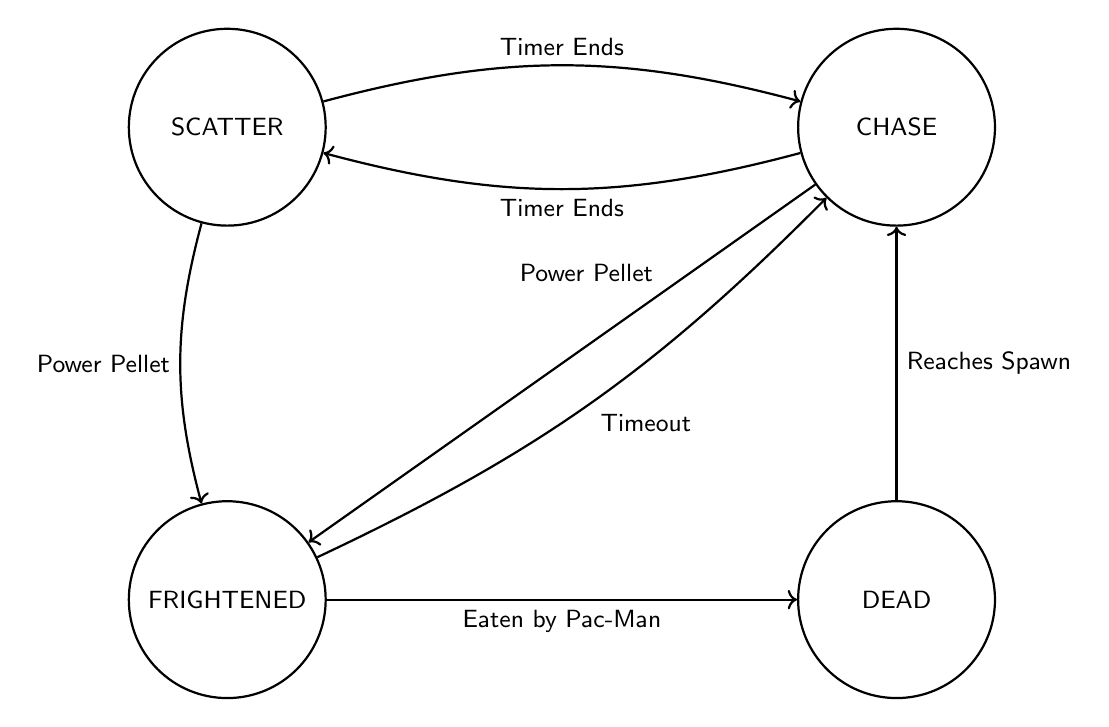
\begin{tikzpicture}[->, auto, thick,
                        every node/.style={font=\sffamily\small},
                        state/.style={draw, circle, minimum size=2.5cm, align=center}]
        
        % States positioned manually for maximum compatibility
        \node[state] (Scatter) at (0, 0) {SCATTER};
        \node[state] (Chase) at (8.5, 0) {CHASE};
        \node[state] (Frightened) at (0, -6) {FRIGHTENED};
        \node[state] (Dead) at (8.5, -6) {DEAD};

        \path
        (Scatter) edge [bend left=15] node {Timer Ends} (Chase)
        (Chase) edge [bend left=15] node {Timer Ends} (Scatter)
        (Scatter) edge [bend right=15] node [left] {Power Pellet} (Frightened)
        (Chase) edge node [above left, pos=0.3] {Power Pellet} (Frightened)
        (Frightened) edge node [below] {Eaten by Pac-Man} (Dead)
        (Frightened) edge [bend right=10] node [below right] {Timeout} (Chase)
        (Dead) edge node [right] {Reaches Spawn} (Chase);
    \end{tikzpicture}
    } % \resizebox vége
    \caption{Finite State Machine (FSM) of Ghost Behaviors}
    \label{fig:ghost_fsm}
\end{figure}

\clearpage

% --- 7. Unit Testing ---
\section{Unit Testing}
The project must include a minimum of \textbf{10 automated JUnit 5 tests}. These tests must strictly focus on the core logical components (the Model layer, such as \texttt{GameEngine} and \texttt{Labyrinth}) without instantiating the Swing graphical user interface.

Every test case must follow the industry-standard \textbf{Arrange-Act-Assert (Given-When-Then)} methodology:
\begin{itemize}
    \item \textbf{Arrange (Given):} Initialize the \texttt{GameEngine}, load a controlled, minimalist test map matrix, and position the entities manually.
    \item \textbf{Act (When):} Trigger a specific game mechanic (e.g., execute a movement command, run one \texttt{step()}, or force a collision). Tests call \texttt{step()} rather than \texttt{update()}, because a test checks a game rule, not the timing; and they create the engine with a fixed-seed \texttt{Random}, so the ghosts' ``random'' choices are the same on every run.
    \item \textbf{Assert (Then):} Verify the expected changes in the game state using JUnit \texttt{Assertions} (e.g., checking if the score increased, coordinates changed, or ghost states updated).
\end{itemize}

\subsection*{Mandatory Test Scenarios}
The test suite must cover critical gameplay mechanics, including but not limited to:
\begin{itemize}
    \item \textbf{Wall Collision:} \textit{Given} Pac-Man is adjacent to and facing a \texttt{WALL} tile, \textit{When} a move command is processed, \textit{Then} Pac-Man's $(X, Y)$ coordinates must remain unchanged.
    \item \textbf{Dot Consumption:} \textit{Given} Pac-Man moves onto a \texttt{DOT} tile, \textit{When} the engine updates the state, \textit{Then} the score must increase, and the tile must change to \texttt{EMPTY}.
    \item \textbf{Ghost Frightened Transition:} \textit{Given} Pac-Man consumes a \texttt{POWERPELLET}, \textit{When} the collision is resolved, \textit{Then} all ghosts must transition from \texttt{CHASE}/\texttt{SCATTER} to the \texttt{FRIGHTENED} state.
    \item \textbf{Death Mechanic:} \textit{Given} Pac-Man and a \texttt{CHASE} ghost stand on the same tile (or swap tiles during one step), \textit{When} collisions are evaluated, \textit{Then} the player's life counter must decrease by 1, and the positions must reset to their respective spawn points.
    \item \textbf{Game Over:} \textit{Given} Pac-Man has one life left, \textit{When} he collides with a \texttt{CHASE} ghost, \textit{Then} \texttt{isGameOver()} must be true, and further steps must not move any figure.
\end{itemize}
\clearpage

% --- 8. I/O and Persistence Contract ---
\section{I/O and Persistence Contract}
The application is following these persistance protocols in order to ensure robust data handling:

\subsection*{1. High-Score Table}
\begin{itemize}
    \item \textbf{File:} \texttt{highscores.csv}
    \item \textbf{Responsibility:} Handled by the \texttt{LevelManager} class, which serves as the general I/O utility for the application.
    \item \textbf{Data Structure:} Each line must strictly follow the format: \texttt{PlayerName;Score;Date}.
    \item \textbf{Player Identity:} The system must not interrupt the player with a text input prompt to ask for their name. Instead, it must automatically fetch the identity of the user currently logged into the operating system using \texttt{System.getProperty("user.name")}.
\end{itemize}

\subsection*{2. Active Game State}
Saving the complex state of an ongoing game (the exact position of Pac-Man, the current \texttt{GhostState} of every ghost, the remaining Frightened timer, the active level, and the state of every individual dot on the map) into a plain text file would require highly error-prone parsing. 

Therefore, the active game state is saved using \textbf{Java Binary Serialization}:
\begin{itemize}
    \item \textbf{File:} \texttt{savestate.dat}
    \item \textbf{Implementation:} All Core Model classes (\texttt{GameEngine}, \texttt{Labyrinth}, \texttt{GameObject}, \texttt{PacMan}, \texttt{Ghost}, the \texttt{GhostStrategy} implementations, and data Enums) must implement the \texttt{java.io.Serializable} interface. \texttt{LevelData} is only passed from the \texttt{LevelManager} to the \texttt{GameEngine} and is not saved, so it does not need to. The engine's \texttt{java.util.Random} is itself serializable, and the plain counters (\texttt{tickInStep}, \texttt{stepCount}) and every figure's start and previous tile are saved automatically.
    \item \textbf{Execution:} The \texttt{GameEngine.saveGameState()} method writes the entire engine instance to a binary file using an \texttt{ObjectOutputStream}. Loading a game simply reads the object back into memory using an \texttt{ObjectInputStream}, perfectly restoring the exact state without manual data mapping.
\end{itemize}

\subsection*{3. Maps}
\label{sec:custom_maps}
\begin{itemize}
    \item \textbf{Format:} Both the built-in levels and the maps made in the \texttt{MapEditor} are plain-text files that look like the maze itself: one maze row per line, one character per tile. The \texttt{LevelManager} reads them line by line with \texttt{loadFromCSV} and writes them with \texttt{saveToCSV}. The built-in first level is \texttt{maps/level1.txt}; the path is relative, so the game must be started from the project folder.
    \item \textbf{Symbols:}

    \vspace{0.2cm}
    \begin{tabular}{@{}cll@{}}
        \toprule
        \textbf{Character} & \textbf{Meaning} & \textbf{Stored as} \\
        \midrule
        \texttt{\#} & Wall & \texttt{CellType.WALL} \\
        \texttt{.} & Dot & \texttt{CellType.DOT} \\
        \texttt{o} & Power pellet & \texttt{CellType.POWERPELLET} \\
        \texttt{\_} & Empty floor & \texttt{CellType.EMPTY} \\
        \texttt{P} & Pac-Man's start tile (exactly one) & \texttt{PacMan} on an \texttt{EMPTY} tile \\
        \texttt{T} & Start tile of a \texttt{TRACKER} ghost & \texttt{Ghost} on an \texttt{EMPTY} tile \\
        \texttt{A} & Start tile of an \texttt{AMBUSHER} ghost & \texttt{Ghost} on an \texttt{EMPTY} tile \\
        \texttt{W} & Start tile of a \texttt{WANDERER} ghost & \texttt{Ghost} on an \texttt{EMPTY} tile \\
        \texttt{C} & Start tile of a \texttt{CHAOTIC} ghost & \texttt{Ghost} on an \texttt{EMPTY} tile \\
        \bottomrule
    \end{tabular}
    \vspace{0.2cm}

    \item \textbf{Why characters instead of \texttt{CellType} names:} A \texttt{CellType} matrix can only describe tiles, so it has no way to record where Pac-Man and the ghosts start. The character picture stores both, stays readable, and can be edited by hand. The ghosts' start tiles also mark the Ghost House, where \texttt{DEAD} ghosts return.
    \item \textbf{Validation:} Every row must have the same length, exactly one \texttt{P} is required, and any other character (including a space) is rejected with its line and column. Empty lines and spaces at the end of a line are ignored, which is why empty floor is written as \texttt{\_} and not as a space.
    \item \textbf{Example} (a small maze with Pac-Man, a power pellet, and two ghosts):

    \vspace{0.1cm}
\begin{verbatim}
#########
#P..o...#
#.##_##.#
#..T_A..#
#########
\end{verbatim}
\end{itemize}

\end{document}